% Scalar instruction entry source: tools/generate_scalar_instruction_catalog.py.
\subsection{\texttt{SW.OR}}
\label{sec:scalar-sw_or}
\index{SW.OR@\texttt{SW.OR}}
\begin{sloppypar}\noindent\textbf{Purpose.} Atomic read-modify-write operation that updates memory without returning a value.\end{sloppypar}\smallskip
\noindent\textbf{Syntax.}\par
\begin{lstlisting}[style=ptoscalarcode]
sw.or<.{rl, f, rlf}> [SrcL], SrcR
\end{lstlisting}
\noindent\textbf{Encoding.}\par
\noindent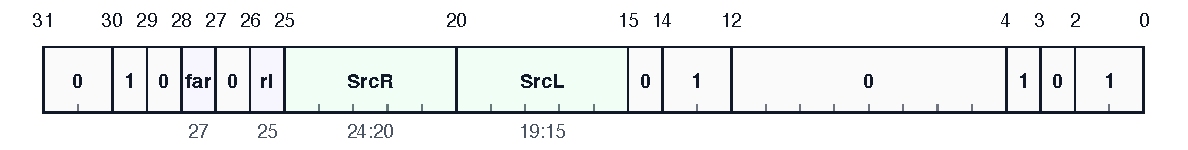
\includegraphics[width=\textwidth]{figs/encoding/scalar_instruction_entries/enc_sw_or.pdf}\par\smallskip
\begin{description}[leftmargin=0.18\linewidth,style=nextline]
\item[Format] \texttt{L32} \texttt{32-bit} scalar word.
\item[Pattern] \texttt{0010.0...........011000000001011}.
\end{description}
\noindent\textbf{Classification.}\par
\begin{description}[leftmargin=0.18\linewidth,style=nextline]
\item[Category] Atomic Memory Operations.
\item[Family] Atomic Operation.
\item[Execution class] \texttt{AMO}; uop\_kind=AMO.
\end{description}
\noindent\textbf{Operand fields.}\par
\begin{description}[leftmargin=0.18\linewidth,style=nextline]
\item[\texttt{SrcL}] Bits \texttt{19:15 (5b)}. 5-bit scalar source register containing the memory address for the atomic read-modify-write operation.
\item[\texttt{SrcR}] Bits \texttt{24:20 (5b)}. 5-bit scalar source register containing the update operand for the atomic read-modify-write operation.
\item[\texttt{far}] Bits \texttt{27:27 (1b)}. Atomic ordering-domain qualifier used with aq/rl suffixes; the assembly suffix containing f selects this encoded bit.
\item[\texttt{rl}] Bits \texttt{25:25 (1b)}. Release ordering bit for atomic memory operations. When set, earlier memory operations cannot be observed after this operation in the selected ordering domain.
\end{description}
\noindent\textbf{Operation.}\par
\begin{lstlisting}[style=ptoscalarcode]
addr = Read(SrcL)
old = AtomicLoad32(addr)
new = old | Read(SrcR)
AtomicStore32(addr, new)
\end{lstlisting}
\Needspace{0.08\textheight}
